% Standalone wrapper to export Figure 1 (the diversity-metric pipeline) as an
% image for the poster/slide. The tikzpicture below is copied VERBATIM from
% paper/sections/01_motivation_workshop.tex (lines 24-75). Libraries match the
% paper preamble (main_icml_workshop.tex line 40). \textwidth is pinned to the
% ICML two-column width so the relative node widths reproduce the paper layout.
% No standalone.cls / preview.sty in this TeX dist, so render on a borderless
% article page and auto-trim the surrounding whitespace (trim_whitespace.py).
\documentclass{article}
\usepackage[paperwidth=22cm,paperheight=24cm,margin=8mm]{geometry}
\usepackage[T1]{fontenc}
\usepackage{amsmath}
\usepackage{amssymb}
\usepackage{tikz}
\usetikzlibrary{positioning, arrows.meta, fit, backgrounds, calc, shapes.geometric}
\pagestyle{empty}
\begin{document}
\noindent
\setlength{\textwidth}{17cm}
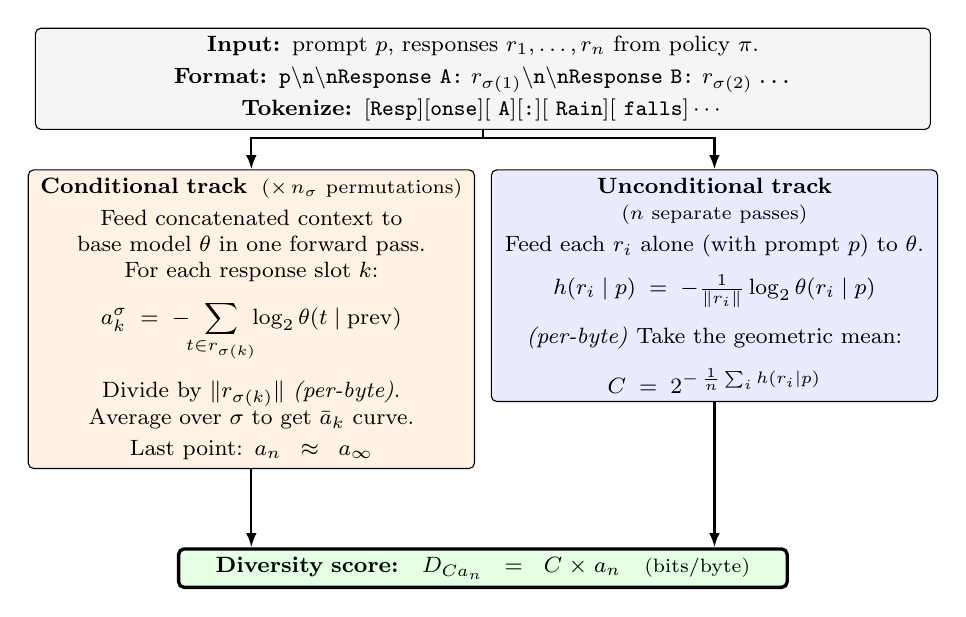
\begin{tikzpicture}[
    font=\footnotesize,
    box/.style={draw, rounded corners=2pt, align=center, inner sep=3pt},
    stage/.style={box, fill=gray!8},
    cond/.style={box, fill=orange!10},
    uncond/.style={box, fill=blue!8},
    final/.style={box, fill=green!10, very thick},
    arrow/.style={-{Latex[length=1.8mm]}, thick},
    node distance=2mm and 4mm,
]

% --- INPUT + FORMAT (combined, top) ---
\node[stage, text width=0.92\textwidth] (input) {
    \textbf{Input:} prompt $p$, responses $r_1,\ldots,r_n$ from policy $\pi$.\\[2pt]
    \textbf{Format:} \texttt{p\textbackslash n\textbackslash nResponse A: $r_{\sigma(1)}$\textbackslash n\textbackslash nResponse B: $r_{\sigma(2)}$\,\ldots}\\[2pt]
    \textbf{Tokenize:} $[\texttt{Resp}][\texttt{onse}][\texttt{ A}][\texttt{:}][\texttt{ Rain}][\texttt{ falls}]\cdots$
};

% --- CONDITIONAL TRACK (LEFT) ---
\node[cond, below left=5mm and 1mm of input.south, text width=0.45\textwidth, anchor=north east] (cond) {
    \textbf{Conditional track} \;{\scriptsize ($\times\,n_\sigma$ permutations)}\\[2pt]
    Feed concatenated context to base model $\theta$ in one forward pass.\\
    For each response slot $k$:
    \[ a_k^\sigma \;=\; -\!\!\sum_{t \in r_{\sigma(k)}}\!\!\log_2 \theta(t \mid \mathrm{prev}) \]
    Divide by $\|r_{\sigma(k)}\|$ \emph{(per-byte)}.\\
    Average over $\sigma$ to get $\bar{a}_k$ curve.\\[2pt]
    Last point: $a_n \approx a_\infty$
};

% --- UNCONDITIONAL TRACK (RIGHT) ---
\node[uncond, below right=5mm and 1mm of input.south, text width=0.45\textwidth, anchor=north west] (unc) {
    \textbf{Unconditional track} \;{\scriptsize ($n$ separate passes)}\\[2pt]
    Feed each $r_i$ alone (with prompt $p$) to $\theta$.
    \[ h(r_i\mid p) \;=\; -\tfrac{1}{\|r_i\|}\log_2 \theta(r_i \mid p) \]
    \emph{(per-byte)} Take the geometric mean:
    \[ C \;=\; 2^{-\,\frac{1}{n}\sum_i h(r_i\mid p)} \]
};

% Arrows from input down to each track
\draw[arrow] (input.south) -- ++(0,-1mm) -| (cond.north);
\draw[arrow] (input.south) -- ++(0,-1mm) -| (unc.north);

% --- FINAL FORMULA ---
\node[final, below=4mm of input, text width=0.62\textwidth, yshift=-49mm] (out) {
    \textbf{Diversity score:}\quad $D_{Ca_n} \;=\; C \times a_n$\quad{\scriptsize(bits/byte)}
};

% Arrows from each track straight down into the final box
\draw[arrow] (cond.south) -- (cond.south |- out.north);
\draw[arrow] (unc.south)  -- (unc.south |- out.north);

\end{tikzpicture}
\end{document}
